% Created 2016-01-20 Wed 11:06
\documentclass{scrartcl}
\usepackage[utf8]{inputenc}
\usepackage[T1]{fontenc}
\usepackage{fixltx2e}
\usepackage{graphicx}
\usepackage{longtable}
\usepackage{float}
\usepackage{wrapfig}
\usepackage{soul}
\usepackage{textcomp}
\usepackage{marvosym}
\usepackage{wasysym}
\usepackage{latexsym}
\usepackage{amssymb}
\usepackage{hyperref}
\tolerance=1000
\usepackage{khpreamble}
\usepackage{subfigure}
\providecommand{\alert}[1]{\textbf{#1}}

\title{Computerized control - homework 1}
\author{Kjartan Halvorsen}
\date{Due 2016-01-22}
\hypersetup{
  pdfkeywords={},
  pdfsubject={},
  pdfcreator={Emacs Org-mode version 7.9.3f}}

\begin{document}

\maketitle



\section{Exercise}
\label{sec-1}
\subsection{Block-diagram calculation}
\label{sec-1-1}

   The block-diagram below shows a so-called \emph{two-degrees-of-freedom} feedback control system. Calculate the transfer function from each of the signals  $u_c$ (command signal), $d$ (disturbance signal) and $n$ (measurement noise) to the system output $y$.

   \begin{center}
   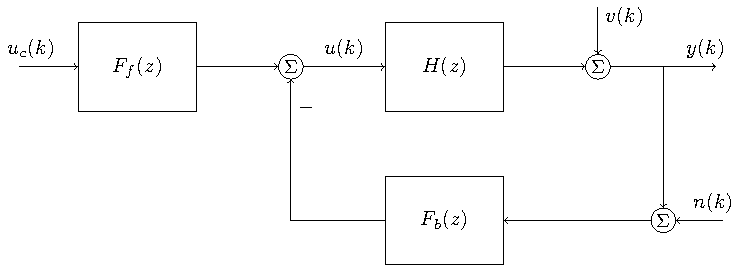
\includegraphics[width=0.6\linewidth]{2dof-block-complete}
   \end{center}
\subsection{Solution to a first-order system}
\label{sec-1-2}

   Consider the first-order system
   \[ \dot{x}(t) = -x(t) + u(t) \]

\begin{enumerate}
\item Write the solution to the system for the input signal 
      \begin{displaymath}
        u(t) = \begin{cases} 1, & 0 \le t \le 1\\ 0, & \text{otherwise}.
      \end{displaymath}
      The initial value is $x(t) = 0$.
\item Sketch the solution $x(t)$ for $0\le t \le 4$, (or generate the plot on the computer).
\item On Blackboard you can find a simulink-file with an implementation of the system. Use this to verify your solution. Include a screen-dump of the simulation output in your report.
\end{enumerate}
\section{Solution}
\label{sec-2}
\subsection{Block-diagram}
\label{sec-2-1}

   One alternative is to use \href{https://en.wikipedia.org/wiki/Mason%2527s_gain_formula}{Mason's rule}. Note that the denominator of the closed-loop transfer functions will be
   \[ 1 + GF_b. \] The numerators are given by the direkt path from the respective input to the output, so we get
   \begin{align*}
   \frac{Y}{U_c} &= \frac{GF_f}{1+GF_b}\\
   \frac{Y}{D} &= \frac{1}{1+GF_b}\\
   \frac{Y}{N} &= -\frac{GF_b}{1+GF_b}
   \end{align*}

   The other alternative is to compute directly in the given block-diagram. We get
   \[ Y = D + G\big(F_fU_c - F_b(N+Y)\big). \]
   Moving terms with $Y$ on the left hand side we get
   \[ Y+GF_bY = D + GF_fU_c - GF_bN. \]
   Deviding by \(1+GF_b\) on both sides gives
   \[ Y = \frac{1}{1+GF_b}D + \frac{GF_f}{1+GF_b}U_c - \frac{GF_b}{1+GF_b}N. \]
\subsection{First-order system}
\label{sec-2-2}

\begin{enumerate}
\item The system can be solved by direct integration of the differential equation, or using the Laplace transform. 

      Using Laplace, we write the input as the sum of two step signals, of which the second is delayed. The solution is then given by summing the solution to each of the two step signals. Write the input as
      \[ u(t) = u_1(t) + u_2(t), \]
      with 
      \begin{align*}
          u_1(t) &= \begin{cases} 1, t \ge 0 \\ 0, & \text{otherwise} \end{cases}\\
          U_1(s) &= \frac{1}{s}.\\
          u_2(t) &= -u_1(t-1) = \begin{cases} -1, t \ge 1 \\ 0, & \text{otherwise} \end{cases}\\ 
          U_2(s) &= -\mexp{-s}U_1(s) = \frac{\mexp{-s}}{s}
      \end{align*}
      Solving using the Laplace transform we get 
      \[ sX = -X + U_1 + U_2\]
      which gives
      \begin{align*}
        X &= \frac{1}{s+1}\left( \frac{1}{s} - \frac{\mexp{-s}{s} \right)\\
          &= \frac{1}{(s+1)s} - \mexp{-s} \frac{1}{(s+1)s},
      \end{align*}
      The first term is a unit step-response, and the second term is also a unit step response, but delayed and with negative sign. The step-response for the system is given by 
      \[ x_1(t) = h(t)(1-\mexp{-t}), \]
      where $h(t)$ is the Heaviside step-function. So the solution is 
      \[ x(t) = x_1(t) + x_2(t) = x_1(t) - x_1(t-1) = h(t)(1 -\mexp{-t}) - h(t-1)\big(1 - \mexp{-(t-1)}\big). \]

      We can also solve the differential equation by integration using the solution
      \[ x(t) = x(0)\mexp{-t} + \int_0^t \mexp{-(t-\tau)} u(\tau) d\tau \]
      Since \(u(t)\) is equal to 1 for \(0\le t< 1\) and zero elsewhere, the integration is quite simple. For $t<1$ we get (since \(x(0) = 0\)) 
      \[ x(t) = \int_0^t \mexp{-t+\tau}d\tau  
              = \int_{-t}^{0} \mexp{\tau'} d\tau' = \left[ \mexp{\tau'} \right]_{-t}^{0} = 1-\mexp{-t}. \]
      And for $t>1$ we get 
      \[ x(t) = \int_0^1 \mexp{-t+\tau}d\tau  
              = \int_{-t}^{-t+1} \mexp{\tau'} d\tau' = \left[ \mexp{\tau'} \right]_{-t}^{-t+1} = \mexp{-t+1}-\mexp{-t}. \]
      So,
      \[ x(t) = \begin{cases} 0, & t \le 0\\
                              1-\mexp{-t}, & 0<t\le 1\\
                              \mexp{-t+1}-\mexp{-t}, & t>1 \end{cases} \]
\item Plot of the solution
      \begin{center}
      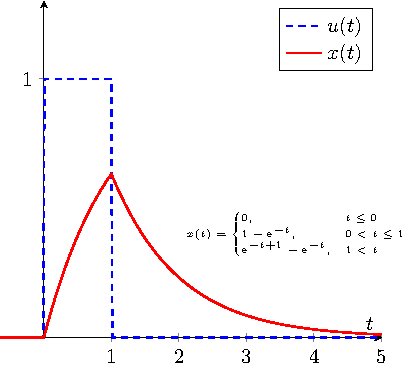
\includegraphics{first-order-response-bb}
      \end{center}
\item Simulink-model with simulation
      \begin{center}
      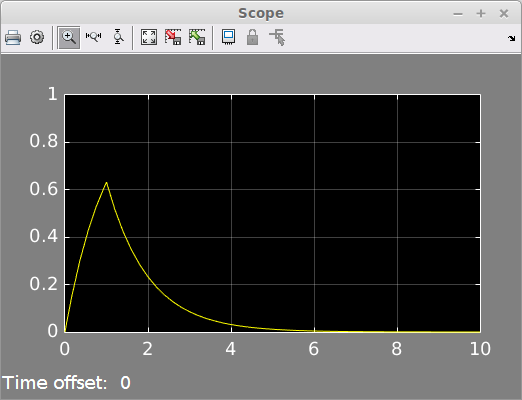
\includegraphics[width=0.5\linewidth]{first-order-simulink}
      \end{center}
\end{enumerate}


     


     
      

\end{document}
